
\section*{1551 finals practice}
\section*{Differential Calculus (Georgia Institute of Technology)}
Math 1551 Version A Name (Print Clearly):\\
Fall 2023\\
Final Exam\\
GT ID Number:\\
Time Limit: 170 Minutes

By signing here, you agree to abide by the Georgia Tech Honor Code:\\
I commit to uphold the ideals of honor and integrity by refusing to betray the trust bestowed upon me as a member of the Georgia Tech Community.

Sign Your Name:\\
This exam contains 33 problems, all multiple choice and weighted equally. Check to see if any pages are missing. Enter all requested information on the top of this page.

You will submit your answers to this exam by filling in the corresponding bubbles on the separate bubble sheet. No partial credit will be given, and no credit will be given for answers in this booklet but incorrectly recorded on the bubble sheet.\\
Please double check your work and your answer choices very carefully.\\
You may not use your books, notes, or any calculator on this exam. You may not receive any assistance with the exam or communicate with others about the problems until it has been graded and returned to you on Gradescope.

Please read the following carefully:

\begin{itemize}
  \item This exam is double-sided.
  \item Each question on this exam has exactly one correct answer. If two answers are selected for any question, it will be marked incorrect.
  \item Do not cut apart, tear apart, or in any other way remove any pages from this exam packet.
  \item If you need extra space, you may use the back side of this cover page.
  \item Take a deep breath and write yourself an encouraging message before you start- you've learned a lot this semester! Thanks for being in our course, and have a great break.
\end{itemize}

\section*{SCRATCH WORK}
\begin{enumerate}
  \item Let $f(x)=x^{2 / 3}(x-5)$. Find all critical points of $f(x)$ on the interval $(-\infty, \infty)$.\\
A. 0 and 2\\
B. 2 only\\
C. 0 only\\
D. 1 and 3\\
E. None of the above
  \item Rolle's Theorem applies to the function $f(x)$ graphed below on the interval $[a, b]$ because...\\
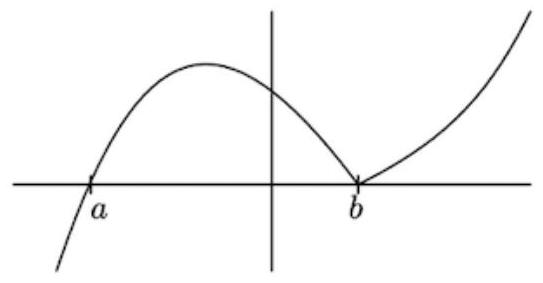
\includegraphics[width=\textwidth]{./images/2025_07_12_b829b47d4ca0804de510g-04}\\
A. $f(x)$ is continuous on $[a, b]$.\\
B. $f(x)$ is differentiable on $(a, b)$.\\
C. $f(a)=f(b)=0$.\\
D. All three statements A, B and C.\\
E. None of these.
  \item Let
\end{enumerate}

$$
f(x)= \begin{cases}\frac{x^{2}+x}{x} & \text { if } x \neq 0 \\ 0 & \text { if } x=0\end{cases}
$$

Select which one of the following statements is true.\\
A. $f(x)$ is continuous at $x=0$.\\
B. $f(x)$ has a removable discontinuity at $x=0$.\\
C. $f(x)$ has a jump discontinuity at $x=0$.\\
D. $f(x)$ has a vertical asymptote at $x=0$.\\
E. None of the other statements are true.

For questions $4-5$, indicate on your bubble sheet which of the options in Antiderivative Bank A is the correct antiderivative of the function (with respect to $x$ ). Each option will be used at most once, and not all options will be used.

Antiderivative Bank A:\\
A. $\frac{x^{4}}{4}+\frac{3^{x}}{\ln (3)}+C$\\
B. $3 \cos (3 x)+\frac{3}{2} x^{2}+C$\\
C. $3 x^{2}+\ln (3) \cdot 3^{x}+C$\\
D. $-\frac{1}{3} \cos (3 x)+\frac{3}{2} x^{2}+C$\\
E. $-\frac{1}{3} \cos (3 x)+\frac{3^{x}}{\ln (3)}+C$\\
4. $f(x)=x^{3}+3^{x}$\\
5. $g(x)=\sin (3 x)+3 x$\\
6. Which one of the following choices is a necessarily true statement involving the Intermediate Value Theorem (IVT) for the function $f(x)$ on the interval $[a, b]$ ?\\
A. If $f(a)<0$ and $f(b)>0$, then by the IVT, $f(x)$ has at least one root on $[a, b]$\\
B. If $f(a)>0$ and $f(b)>0$, then by the IVT, $f(x)$ cannot have any roots on $[a, b]$\\
C. If $f(x)$ is continuous and has at least one root on $[a, b]$, then by the IVT, $f(a)$ and $f(b)$ have opposite signs\\
D. If $f(x)$ is discontinuous somewhere on $[a, b]$, then by the IVT, it cannot have any roots on $[a, b]$\\
E. If $f(x)$ is continuous and has no roots on $[a, b]$, then by the IVT, $f(a)$ and $f(b)$ must have the same sign\\
7. Consider the function $f(x)=x^{2}$ on the interval $[0,3]$. The value of $c$ in the interval guaranteed to exist by the Mean Value Theorem is:\\
A. 1\\
B. 2\\
C. $\frac{3}{2}$\\
D. $\frac{1}{2}$\\
E. None of these\\
8. Let $f(x)=x^{3}-6 x^{2}+9 x-2$. Where does $f(x)$ achieve a local maximum on $[0,4]$ ?\\
A. $x=1$ and $x=3$\\
B. $x=1$ and $x=4$\\
C. $x=1$ only\\
D. $x=0$ and $x=3$\\
E. $x=0$ and $x=4$\\
9. Let $f(x)=x^{3}-6 x^{2}+9 x-2$. On which intervals is $f$ concave up?\\
A. $(-\infty, 2)$\\
B. $(-\infty, 1)$ and $(3, \infty)$\\
C. $(1,3)$\\
D. $(-\infty, 2)$ and $(2, \infty)$\\
E. $(2, \infty)$\\
10. Which of the following is a correct expression for $f^{\prime}(0)$, where $f(x)=\ln (x+1)$ ?\\
A. $\lim _{h \rightarrow 0} \frac{\ln (h+1)}{h}$\\
B. $\lim _{h \rightarrow 0} \frac{\ln (h+1)-1}{h}$\\
C. $\lim _{x \rightarrow 0} \frac{\ln (x+1)}{h}$\\
D. $\lim _{h \rightarrow 0} \frac{\ln (x+h+1)-\ln (x+1)}{h}$\\
E. None of the above\\
11. Which of the following is the equation of the line tangent to $f(x)=2 e^{3 x}$ at $x=0$ ?\\
A. $y=2+3 x$\\
B. $y=2+6 x$\\
C. $y=3+6 x$\\
D. $y=2 e+6 e x$\\
E. $y=3 e^{x}+6 x e^{x}$\\
12. Consider the piecewise-defined function

$$
f(x)=\left\{\begin{array}{l}
3 x^{2}+b x \text { if } x<1 \\
2 x+a \text { if } x \geq 1
\end{array}\right.
$$

Which one of the following choices correctly describes values for $b$ and $a$ that will make $f(x)$ differentiable on $(-\infty, \infty)$ ?\\
A. $a=-2, b=-6$\\
B. $a=-3, b=-4$\\
C. $a=-4, b=-5$\\
D. $f(x)$ will be differentiable on $(-\infty, \infty)$ for any choice of $a$ and $b$\\
E. $f(x)$ will not be differentiable on $(-\infty, \infty)$ for any choice of $a$ or $b$\\
13. Which one of the following statements is sufficient to prove that the line $y=a$ is a horizontal asymptote of the function $f(x)$ ?\\
A. $\lim _{x \rightarrow a^{+}} f(x)=\infty$\\
B. $\lim _{x \rightarrow a^{-}} f(x)=-\infty$\\
C. $\lim _{x \rightarrow \infty} f(x)=\infty$\\
D. $\lim _{x \rightarrow-\infty} f(x)=a$\\
E. $\lim _{x \rightarrow-\infty} f(x)=\infty$\\
14. The diagram shows the graph of a function $f(x)$. If we apply Newton's method to approximate a solution of $f(x)=0$ using $x_{0}=1$, what is $x_{1}$ ?\\
A. -1\\
B. 0\\
C. 1\\
D. 2\\
E. 3\\
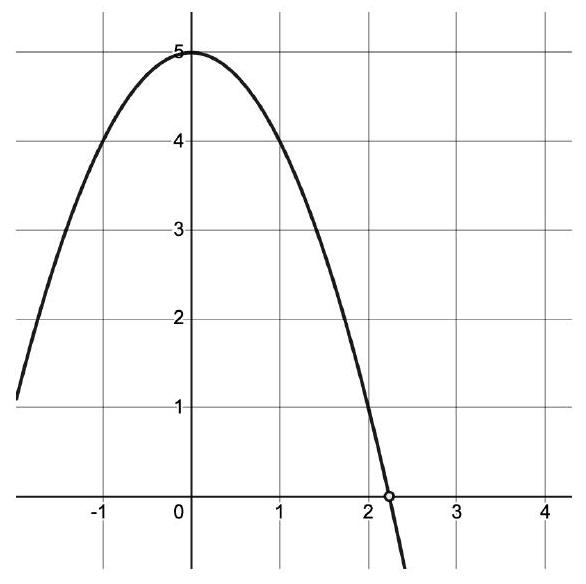
\includegraphics[width=\textwidth]{./images/2025_07_12_b829b47d4ca0804de510g-07}\\
15. Consider finding the root of $f(x)=x^{2}-4$ using Newton's method. If you start with $x_{0}=3$, after one iteration of the method, what is $x_{1}$ ?\\
A. $x_{1}=2$\\
B. $x_{1}=\frac{13}{6}$\\
C. $x_{1}=\frac{9}{5}$\\
D. $x_{1}=\frac{23}{6}$\\
E. $x_{1}=\frac{7}{6}$

For questions 16-18, indicate on your bubble sheet which of the options in Derivative Bank A is the correct derivative of the function. Each option will be used at most once, and not all options will be used.

Derivative Bank A:\\
A. $\frac{x 2^{x-1}}{1+4 x^{2}}$\\
B. $2^{x}\left[\ln (2) \arctan (2 x)+\frac{2}{1+4 x^{2}}\right]$\\
C. $-\ln (2)\left[\frac{1}{x^{2} \tan (x)}+\frac{1}{x \sin ^{2}(x)}\right]$\\
D. $(2 x)^{x}(\ln (2 x)+1)$\\
E. $(2 x)^{x} \ln (2)-\arctan (2 x)$\\
16. $f(x)=2^{x} \arctan (2 x)$\\
17. $g(x)=(2 x)^{x}$\\
18. $h(x)=\frac{\ln (2)}{x \tan (x)}$

Use the graph of $f(x)$ below to answer questions 1-3.\\
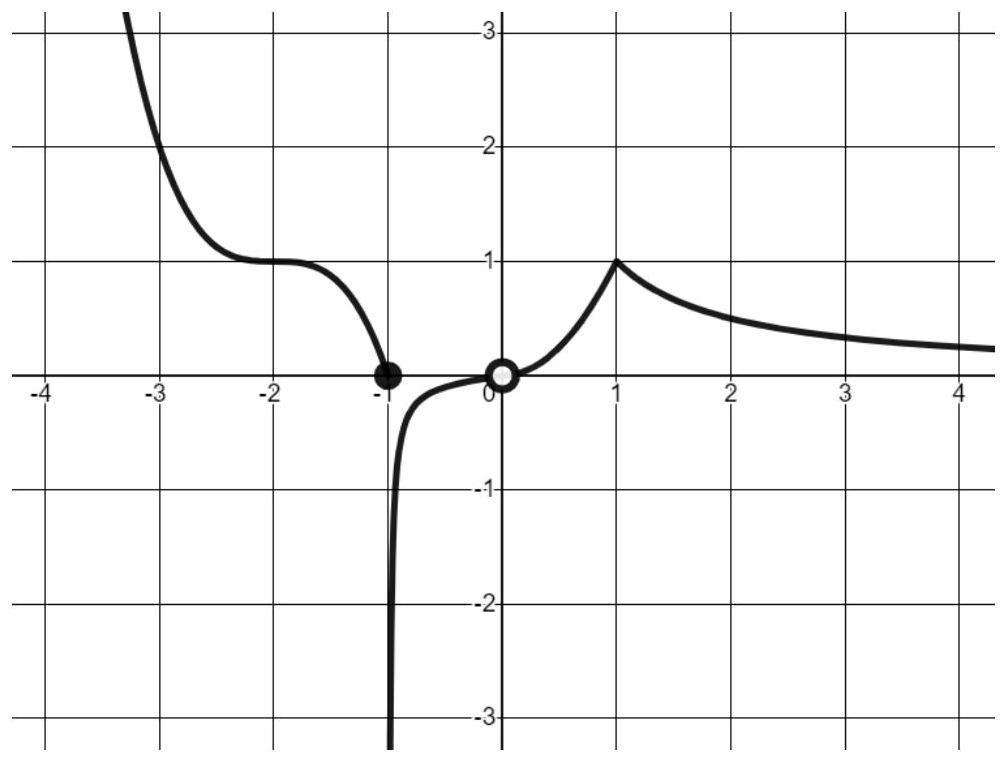
\includegraphics[width=\textwidth]{./images/2025_07_12_b829b47d4ca0804de510g-09}\\
19. Based on the graph, which one of the following statements is true?\\
A. $\lim _{x \rightarrow 0} f(x)=\infty$\\
B. $\lim _{x \rightarrow-1} f(x)=0$\\
C. $\lim _{x \rightarrow-1^{+}} f(x)=-\infty$\\
D. $\lim _{x \rightarrow 1} f(x)$ DNE\\
E. $f(0)=0$\\
20. Based on the graph, which of the following describes $f(x)$ at $x=1$ ?\\
A. Continuous but not differentiable\\
B. Differentiable but not continuous\\
C. Both continuous and differentiable\\
D. Neither continuous nor differentiable\\
E. None of the above\\
21. Based on the graph, choose the value of $a$ such that $\lim _{x \rightarrow a} \frac{f(x)-f(a)}{x-a}$ exists.\\
A. -2\\
B. -1\\
C. 0\\
D. 1\\
E. All of the above\\
22. A large clock is hanging on a vertical wall. A ladybug is resting at the tip of the second hand, which is 1 foot long and is rotating clockwise at a constant rate of $2 \pi$ radians per minute. At the moment when the second hand is pointing exactly at 1 o'clock, how fast is the height of the ladybug changing?\\

\includegraphics[width=\textwidth]{./images/2025_07_12_b829b47d4ca0804de510g-10}\\
A. $-\pi$ feet per minute\\
B. $-\frac{\sqrt{3}}{2} \pi$ feet per minute\\
C. $-\frac{\sqrt{3}}{\pi}$ feet per minute\\
D. $-\sqrt{3} \pi$ feet per minute\\
E. $-2 \pi$ feet per minute\\
23. Which one of the following statements is necessarily true?\\
A. If $\lim _{x \rightarrow a} f(x)$ does not exist, and $\lim _{x \rightarrow a} g(x)$ does not exist, then $\lim _{x \rightarrow a}[f(x)+g(x)]$ does not exist\\
B. If $\lim _{x \rightarrow a} f(x)=M$, and $\lim _{x \rightarrow a} g(x)=N$, then $\lim _{x \rightarrow a} \frac{f(x)}{g(x)}=\frac{M}{N}$\\
C. $\lim _{x \rightarrow a} f(g(x))=f\left(\lim _{x \rightarrow a} g(x)\right)$\\
D. If $f$ is differentiable at $x=a$, and $g$ is continuous at $x=a$, then $\lim _{x \rightarrow a}[f(x) g(x)]=f(a) g(a)$\\
E. None of the above\\
24. Suppose we know that for all values of $x$,

$$
m-x^{2} \leq f(x) \leq 2+m e^{x}
$$

For which of the following values of $m$ can we use the sandwich theorem to calculate $\lim _{x \rightarrow 0} f(x)$ ?\\
A. $m=0$\\
B. $m=1$.\\
C. $m=-1$.\\
D. $m=2$.\\
E. None of the above\\
25. Evaluate $\lim _{x \rightarrow 0} \frac{\sin \left(2 x^{3}\right)}{\sin \left(3 x^{2}\right)}$.\\
A. $\frac{2}{3}$\\
B. 0\\
C. 1\\
D. $\frac{8}{9}$\\
E. $\infty$\\
26. Suppose $f(x)$ is a function where $\lim _{x \rightarrow 2} f(x)=5$, then which of the following must be true?\\
A. $f^{\prime}(2)$ exists.\\
B. $f(x)$ is continuous at $x=2$.\\
C. $f(x)$ is defined at $x=2$.\\
D. $f(2)=5$.\\
E. None of the other statements is necessarily true.\\
27. Which of the following is a linear approximation of $x^{\frac{2}{3}}$ near $x=8$ ? Is the linear approximation an overestimate or underestimate of the function near $x=8$ ?\\
A. $4+\frac{1}{3}(x-8)$, overestimate\\
B. $4+\frac{1}{3}(x-8)$, underestimate\\
C. $6+\frac{4}{3}(x-8)$, overestimate\\
D. $6+\frac{4}{3}(x-8)$, underestimate\\
E. $4+\frac{4}{3}(x-8)$, overestimate

For questions 28-30, indicate on your bubble sheet which of the options in Derivative Bank B is the correct derivative of the function. Each option will be used at most once, and not all options will be used.

Derivative Bank B:\\
A. $\cos (x)-x \sin (x)$\\
B. $\frac{\cos \left(\ln \left(\frac{x}{3}\right)\right)}{x}$\\
C. $\cos (x) \ln \left(\frac{x}{3}\right)+\frac{1}{x} \sin (x)$\\
D. $\frac{1-\ln (x)}{3 x^{2}}$\\
E. $\frac{1}{3 x}$\\
28. $f(x)=x \cos (x)$\\
29. $g(x)=\sin \left(\ln \left(\frac{x}{3}\right)\right)$\\
30. $h(x)=\frac{\ln (x)}{3 x}$\\
31. Suppose the function $f(x)$ is differentiable at the point $x=a$, and that\\
$\mathrm{D}=$ the derivative of $f(x)$ at $x=a$\\
$\mathrm{I}=$ the instantaneous rate of change of $f(x)$ at $x=a$\\
$\mathrm{S}=$ the slope of the tangent line to $f(x)$ at $x=a$

Which of the following correctly describes the relationship between these quantities?\\
A. D and I are equal to each other, but not equal to S\\
B. D and S are equal to each other, but not equal to I\\
C. I and S are equal to each other, but not equal to D\\
D. D, I, and S are all equal to each other\\
E. None of the quantities are necessarily equal to each other\\
32. Consider the curve $2 x^{2}=y^{2}+x y$. Find $\frac{d y}{d x}$.\\
A. $\frac{d y}{d x}=\frac{4 x-y}{2 y+x}$\\
B. $\frac{d y}{d x}=\frac{2 y+x}{4 x-y}$\\
C. $\frac{d y}{d x}=\frac{4 x-y}{2 y-x}$\\
D. $\frac{d y}{d x}=\frac{2 x-y}{y+2 x}$\\
E. None of the above\\
33. Which of the following statements are true of the function graphed below?\\
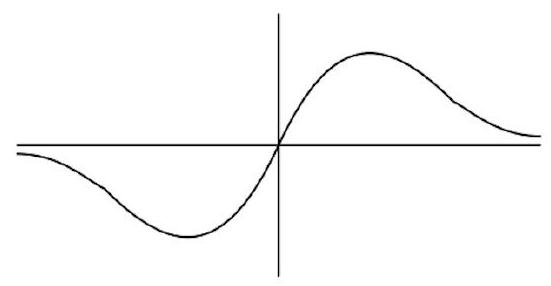
\includegraphics[width=\textwidth]{./images/2025_07_12_b829b47d4ca0804de510g-13}\\
I. There is a horizontal asymptote at $y=0$.\\
II. There are three inflection points.\\
III. There are no absolute extrema.\\
A. I only\\
B. I, II only\\
C. I, III only\\
D. II, III only\\
E. None are true

EXTRA CREDIT: Use the space on the back of your bubble sheet to answer the extra credit problem.\\
Think about one problem/topic you have worked on in this class this semester (from a homework, quiz, worksheet, exam, etc) that you struggled to understand and solve, and explain how the struggle itself was valuable.\\
In the context of this question, describe the struggle and how you overcame it. You should discuss whether struggling built aspects of character in you (e.g. endurance, self-confidence, competence to solve new problems) and how these virtues might benefit you in later ventures. Please note that your answer should include some form of self-reflection in order to attain the 3 \% points. Your answer should be no longer than 3-4 lines.


\end{document}